\documentclass[1p]{elsarticle_modified}
%\bibliographystyle{elsarticle-num}

%\usepackage[colorlinks]{hyperref}
%\usepackage{abbrmath_seonhwa} %\Abb, \Ascr, \Acal ,\Abf, \Afrak
\usepackage{amsfonts}
\usepackage{amssymb}
\usepackage{amsmath}
\usepackage{amsthm}
\usepackage{scalefnt}
\usepackage{amsbsy}
\usepackage{kotex}
\usepackage{caption}
\usepackage{subfig}
\usepackage{color}
\usepackage{graphicx}
\usepackage{xcolor} %% white, black, red, green, blue, cyan, magenta, yellow
\usepackage{float}
\usepackage{setspace}
\usepackage{hyperref}

\usepackage{tikz}
\usetikzlibrary{arrows}

\usepackage{multirow}
\usepackage{array} % fixed length table
\usepackage{hhline}

%%%%%%%%%%%%%%%%%%%%%
\makeatletter
\renewcommand*\env@matrix[1][\arraystretch]{%
	\edef\arraystretch{#1}%
	\hskip -\arraycolsep
	\let\@ifnextchar\new@ifnextchar
	\array{*\c@MaxMatrixCols c}}
\makeatother %https://tex.stackexchange.com/questions/14071/how-can-i-increase-the-line-spacing-in-a-matrix
%%%%%%%%%%%%%%%

\usepackage[normalem]{ulem}

\newcommand{\msout}[1]{\ifmmode\text{\sout{\ensuremath{#1}}}\else\sout{#1}\fi}
%SOURCE: \msout is \stkout macro in https://tex.stackexchange.com/questions/20609/strikeout-in-math-mode

\newcommand{\cancel}[1]{
	\ifmmode
	{\color{red}\msout{#1}}
	\else
	{\color{red}\sout{#1}}
	\fi
}

\newcommand{\add}[1]{
	{\color{blue}\uwave{#1}}
}

\newcommand{\replace}[2]{
	\ifmmode
	{\color{red}\msout{#1}}{\color{blue}\uwave{#2}}
	\else
	{\color{red}\sout{#1}}{\color{blue}\uwave{#2}}
	\fi
}

\newcommand{\Sol}{\mathcal{S}} %segment
\newcommand{\D}{D} %diagram
\newcommand{\A}{\mathcal{A}} %arc


%%%%%%%%%%%%%%%%%%%%%%%%%%%%%5 test

\def\sl{\operatorname{\textup{SL}}(2,\Cbb)}
\def\psl{\operatorname{\textup{PSL}}(2,\Cbb)}
\def\quan{\mkern 1mu \triangleright \mkern 1mu}

\theoremstyle{definition}
\newtheorem{thm}{Theorem}[section]
\newtheorem{prop}[thm]{Proposition}
\newtheorem{lem}[thm]{Lemma}
\newtheorem{ques}[thm]{Question}
\newtheorem{cor}[thm]{Corollary}
\newtheorem{defn}[thm]{Definition}
\newtheorem{exam}[thm]{Example}
\newtheorem{rmk}[thm]{Remark}
\newtheorem{alg}[thm]{Algorithm}

\newcommand{\I}{\sqrt{-1}}
\begin{document}

%\begin{frontmatter}
%
%\title{Boundary parabolic representations of knots up to 8 crossings}
%
%%% Group authors per affiliation:
%\author{Yunhi Cho} 
%\address{Department of Mathematics, University of Seoul, Seoul, Korea}
%\ead{yhcho@uos.ac.kr}
%
%
%\author{Seonhwa Kim} %\fnref{s_kim}}
%\address{Center for Geometry and Physics, Institute for Basic Science, Pohang, 37673, Korea}
%\ead{ryeona17@ibs.re.kr}
%
%\author{Hyuk Kim}
%\address{Department of Mathematical Sciences, Seoul National University, Seoul 08826, Korea}
%\ead{hyukkim@snu.ac.kr}
%
%\author{Seokbeom Yoon}
%\address{Department of Mathematical Sciences, Seoul National University, Seoul, 08826,  Korea}
%\ead{sbyoon15@snu.ac.kr}
%
%\begin{abstract}
%We find all boundary parabolic representation of knots up to 8 crossings.
%
%\end{abstract}
%\begin{keyword}
%    \MSC[2010] 57M25 
%\end{keyword}
%
%\end{frontmatter}

%\linenumbers
%\tableofcontents
%
\newcommand\colored[1]{\textcolor{white}{\rule[-0.35ex]{0.8em}{1.4ex}}\kern-0.8em\color{red} #1}%
%\newcommand\colored[1]{\textcolor{white}{ #1}\kern-2.17ex	\textcolor{white}{ #1}\kern-1.81ex	\textcolor{white}{ #1}\kern-2.15ex\color{red}#1	}

{\Large $\underline{11a_{111}~(K11a_{111})}$}

\setlength{\tabcolsep}{10pt}
\renewcommand{\arraystretch}{1.6}
\vspace{1cm}\begin{tabular}{m{100pt}>{\centering\arraybackslash}m{274pt}}
\multirow{5}{120pt}{
	\centering
	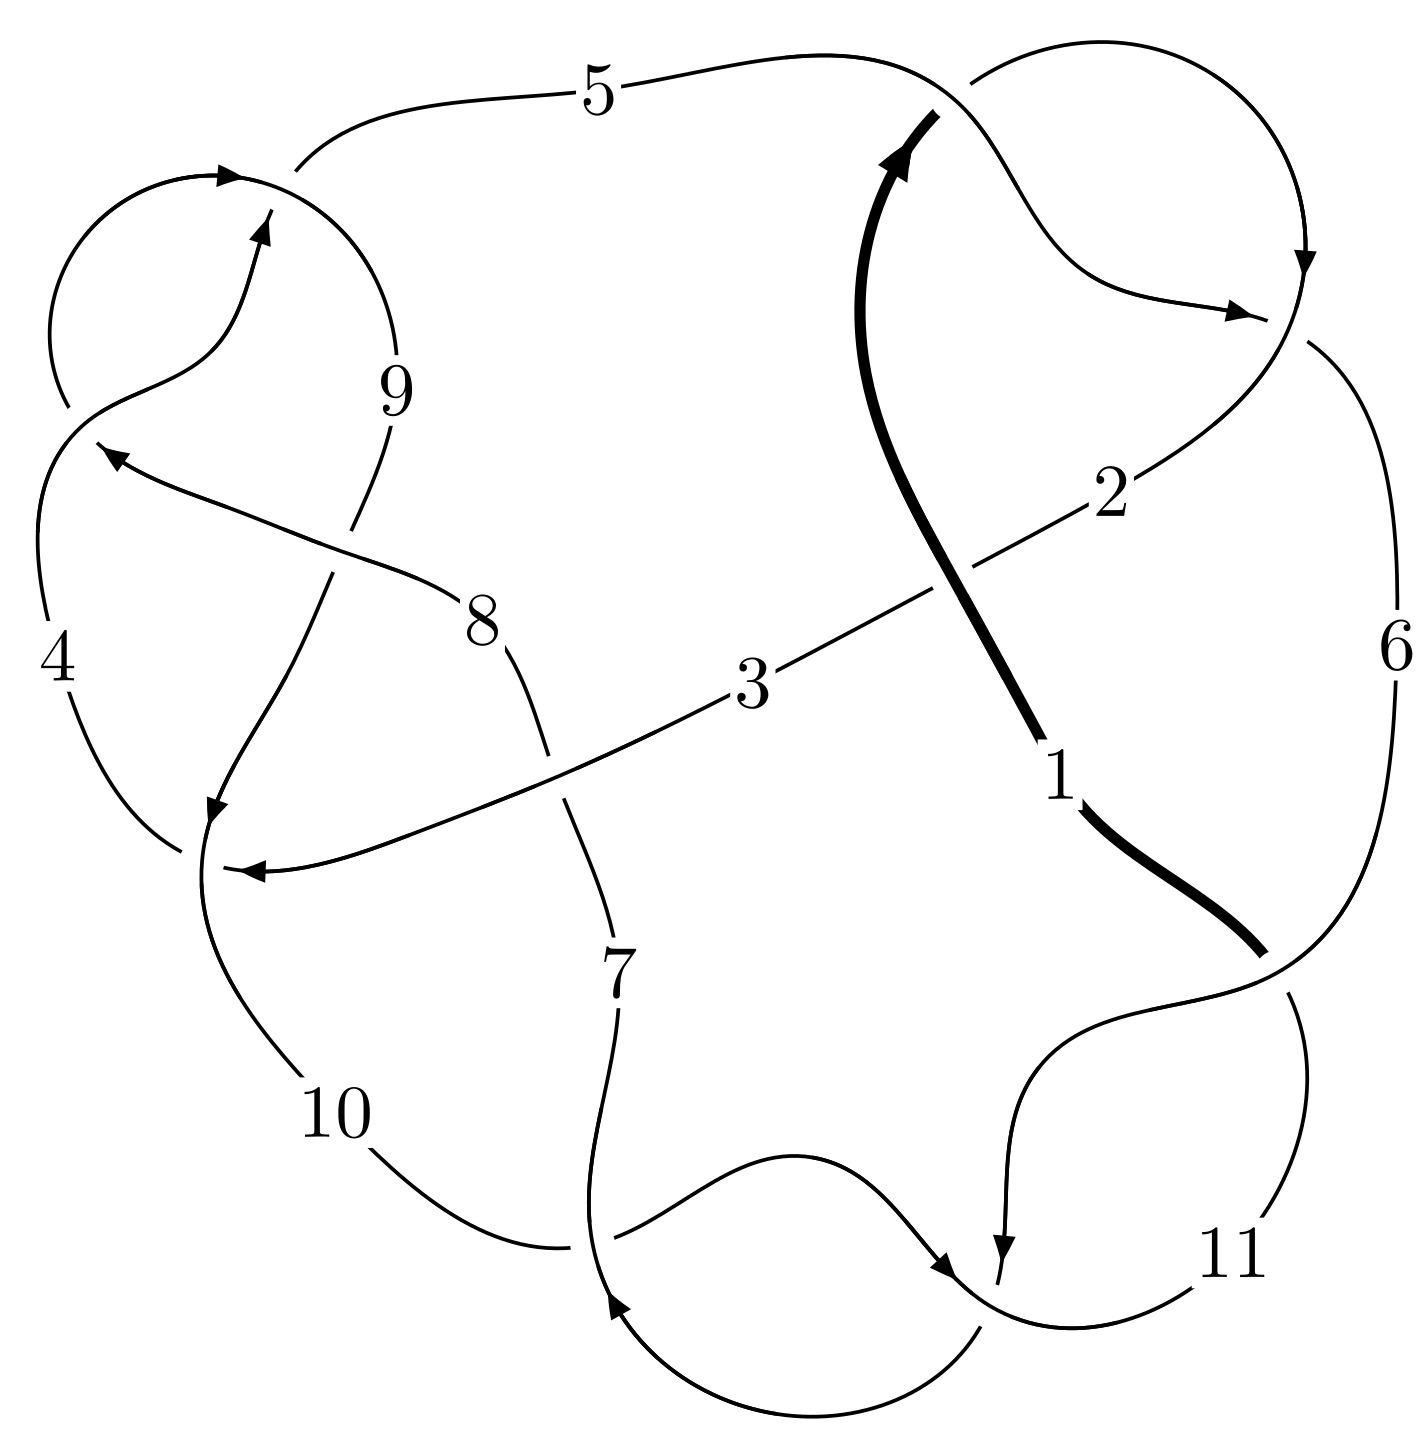
\includegraphics[width=112pt]{../../../GIT/diagram.site/Diagrams/png/360_11a_111.png}\\
\ \ \ A knot diagram\footnotemark}&
\allowdisplaybreaks
\textbf{Linearized knot diagam} \\
\cline{2-2}
 &
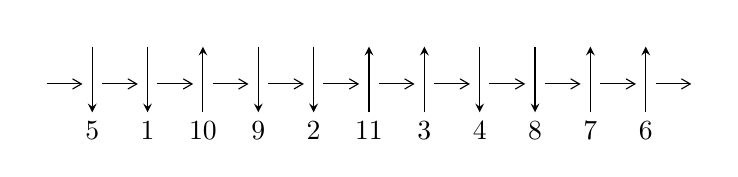
\begin{tikzpicture}[x=20pt, y=17pt]
	% nodes
	\node (C0) at (0, 0) {};
	\node (C1) at (1, 0) {};
	\node (C1U) at (1, +1) {};
	\node (C1D) at (1, -1) {5};

	\node (C2) at (2, 0) {};
	\node (C2U) at (2, +1) {};
	\node (C2D) at (2, -1) {1};

	\node (C3) at (3, 0) {};
	\node (C3U) at (3, +1) {};
	\node (C3D) at (3, -1) {10};

	\node (C4) at (4, 0) {};
	\node (C4U) at (4, +1) {};
	\node (C4D) at (4, -1) {9};

	\node (C5) at (5, 0) {};
	\node (C5U) at (5, +1) {};
	\node (C5D) at (5, -1) {2};

	\node (C6) at (6, 0) {};
	\node (C6U) at (6, +1) {};
	\node (C6D) at (6, -1) {11};

	\node (C7) at (7, 0) {};
	\node (C7U) at (7, +1) {};
	\node (C7D) at (7, -1) {3};

	\node (C8) at (8, 0) {};
	\node (C8U) at (8, +1) {};
	\node (C8D) at (8, -1) {4};

	\node (C9) at (9, 0) {};
	\node (C9U) at (9, +1) {};
	\node (C9D) at (9, -1) {8};

	\node (C10) at (10, 0) {};
	\node (C10U) at (10, +1) {};
	\node (C10D) at (10, -1) {7};

	\node (C11) at (11, 0) {};
	\node (C11U) at (11, +1) {};
	\node (C11D) at (11, -1) {6};
	\node (C12) at (12, 0) {};

	% arrows
	\draw[->,>={angle 60}]
	(C0) edge (C1) (C1) edge (C2) (C2) edge (C3) (C3) edge (C4) (C4) edge (C5) (C5) edge (C6) (C6) edge (C7) (C7) edge (C8) (C8) edge (C9) (C9) edge (C10) (C10) edge (C11) (C11) edge (C12) ;	\draw[->,>=stealth]
	(C1U) edge (C1D) (C2U) edge (C2D) (C3D) edge (C3U) (C4U) edge (C4D) (C5U) edge (C5D) (C6D) edge (C6U) (C7D) edge (C7U) (C8U) edge (C8D) (C9U) edge (C9D) (C10D) edge (C10U) (C11D) edge (C11U) ;
	\end{tikzpicture} \\
\hhline{~~} \\& 
\textbf{Solving Sequence} \\ \cline{2-2} 
 &
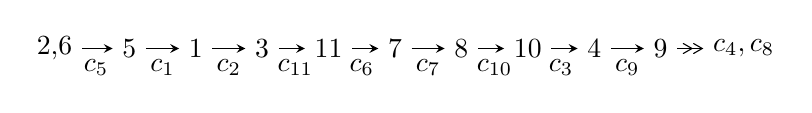
\begin{tikzpicture}[x=24pt, y=7pt]
	% node
	\node (A0) at (-1/8, 0) {2,6};
	\node (A1) at (1, 0) {5};
	\node (A2) at (2, 0) {1};
	\node (A3) at (3, 0) {3};
	\node (A4) at (4, 0) {11};
	\node (A5) at (5, 0) {7};
	\node (A6) at (6, 0) {8};
	\node (A7) at (7, 0) {10};
	\node (A8) at (8, 0) {4};
	\node (A9) at (9, 0) {9};
	\node (C1) at (1/2, -1) {$c_{5}$};
	\node (C2) at (3/2, -1) {$c_{1}$};
	\node (C3) at (5/2, -1) {$c_{2}$};
	\node (C4) at (7/2, -1) {$c_{11}$};
	\node (C5) at (9/2, -1) {$c_{6}$};
	\node (C6) at (11/2, -1) {$c_{7}$};
	\node (C7) at (13/2, -1) {$c_{10}$};
	\node (C8) at (15/2, -1) {$c_{3}$};
	\node (C9) at (17/2, -1) {$c_{9}$};
	\node (A10) at (41/4, 0) {$c_{4},c_{8}$};

	% edge
	\draw[->,>=stealth]	
	(A0) edge (A1) (A1) edge (A2) (A2) edge (A3) (A3) edge (A4) (A4) edge (A5) (A5) edge (A6) (A6) edge (A7) (A7) edge (A8) (A8) edge (A9) ;
	\draw[->>,>={angle 60}]	
	(A9) edge (A10);
\end{tikzpicture} \\ 

\end{tabular} \\

\footnotetext{
The image of knot diagram is generated by the software ``\textbf{Draw programme}" developed by Andrew Bartholomew(\url{http://www.layer8.co.uk/maths/draw/index.htm\#Running-draw}), where we modified some parts for our purpose(\url{https://github.com/CATsTAILs/LinksPainter}).
}\phantom \\ \newline 
\centering \textbf{Ideals for irreducible components\footnotemark of $X_{\text{par}}$} 
 
\begin{align*}
I^u_{1}&=\langle 
u^{51}- u^{50}+\cdots+2 u-1\rangle \\
\\
\end{align*}
\raggedright * 1 irreducible components of $\dim_{\mathbb{C}}=0$, with total 51 representations.\\
\footnotetext{All coefficients of polynomials are rational numbers. But the coefficients are sometimes approximated in decimal forms when there is not enough margin.}
\newpage
\renewcommand{\arraystretch}{1}
\centering \section*{I. $I^u_{1}= \langle u^{51}- u^{50}+\cdots+2 u-1 \rangle$}
\flushleft \textbf{(i) Arc colorings}\\
\begin{tabular}{m{7pt} m{180pt} m{7pt} m{180pt} }
\flushright $a_{2}=$&$\begin{pmatrix}0\\u\end{pmatrix}$ \\
\flushright $a_{6}=$&$\begin{pmatrix}1\\0\end{pmatrix}$ \\
\flushright $a_{5}=$&$\begin{pmatrix}1\\- u^2\end{pmatrix}$ \\
\flushright $a_{1}=$&$\begin{pmatrix}u\\- u^3+u\end{pmatrix}$ \\
\flushright $a_{3}=$&$\begin{pmatrix}- u^3\\u^5- u^3+u\end{pmatrix}$ \\
\flushright $a_{11}=$&$\begin{pmatrix}u^3\\- u^3+u\end{pmatrix}$ \\
\flushright $a_{7}=$&$\begin{pmatrix}u^6- u^4+1\\- u^6+2 u^4- u^2\end{pmatrix}$ \\
\flushright $a_{8}=$&$\begin{pmatrix}u^{14}-3 u^{12}+4 u^{10}- u^8+1\\- u^{16}+4 u^{14}-8 u^{12}+8 u^{10}-4 u^8-2 u^6+4 u^4-2 u^2\end{pmatrix}$ \\
\flushright $a_{10}=$&$\begin{pmatrix}u^9-2 u^7+u^5+2 u^3- u\\- u^9+3 u^7-3 u^5+u\end{pmatrix}$ \\
\flushright $a_{4}=$&$\begin{pmatrix}u^{23}-6 u^{21}+16 u^{19}-20 u^{17}+4 u^{15}+22 u^{13}-26 u^{11}+6 u^9+9 u^7-6 u^5\\- u^{23}+7 u^{21}+\cdots-2 u^3+u\end{pmatrix}$ \\
\flushright $a_{9}=$&$\begin{pmatrix}u^{39}-10 u^{37}+\cdots-7 u^7+6 u^5\\- u^{41}+11 u^{39}+\cdots-2 u^3+u\end{pmatrix}$\\ \flushright $a_{9}=$&$\begin{pmatrix}u^{39}-10 u^{37}+\cdots-7 u^7+6 u^5\\- u^{41}+11 u^{39}+\cdots-2 u^3+u\end{pmatrix}$\\&\end{tabular}
\flushleft \textbf{(ii) Obstruction class $= -1$}\\~\\
\flushleft \textbf{(iii) Cusp Shapes $= -4 u^{50}+60 u^{48}+\cdots+4 u-10$}\\~\\
\newpage\renewcommand{\arraystretch}{1}
\flushleft \textbf{(iv) u-Polynomials at the component}\newline \\
\begin{tabular}{m{50pt}|m{274pt}}
Crossings & \hspace{64pt}u-Polynomials at each crossing \\
\hline $$\begin{aligned}c_{1},c_{5}\end{aligned}$$&$\begin{aligned}
&u^{51}+u^{50}+\cdots+2 u+1
\end{aligned}$\\
\hline $$\begin{aligned}c_{2}\end{aligned}$$&$\begin{aligned}
&u^{51}+29 u^{50}+\cdots+2 u+1
\end{aligned}$\\
\hline $$\begin{aligned}c_{3}\end{aligned}$$&$\begin{aligned}
&u^{51}-3 u^{50}+\cdots+96 u+77
\end{aligned}$\\
\hline $$\begin{aligned}c_{4},c_{8}\end{aligned}$$&$\begin{aligned}
&u^{51}- u^{50}+\cdots- u^2+1
\end{aligned}$\\
\hline $$\begin{aligned}c_{6},c_{10},c_{11}\end{aligned}$$&$\begin{aligned}
&u^{51}+3 u^{50}+\cdots+38 u+5
\end{aligned}$\\
\hline $$\begin{aligned}c_{7}\end{aligned}$$&$\begin{aligned}
&u^{51}+u^{50}+\cdots-15 u^2+25
\end{aligned}$\\
\hline $$\begin{aligned}c_{9}\end{aligned}$$&$\begin{aligned}
&u^{51}+25 u^{50}+\cdots+2 u+1
\end{aligned}$\\
\hline
\end{tabular}\\~\\
\newpage\renewcommand{\arraystretch}{1}
\flushleft \textbf{(v) Riley Polynomials at the component}\newline \\
\begin{tabular}{m{50pt}|m{274pt}}
Crossings & \hspace{64pt}Riley Polynomials at each crossing \\
\hline $$\begin{aligned}c_{1},c_{5}\end{aligned}$$&$\begin{aligned}
&y^{51}-29 y^{50}+\cdots+2 y-1
\end{aligned}$\\
\hline $$\begin{aligned}c_{2}\end{aligned}$$&$\begin{aligned}
&y^{51}-13 y^{50}+\cdots-6 y-1
\end{aligned}$\\
\hline $$\begin{aligned}c_{3}\end{aligned}$$&$\begin{aligned}
&y^{51}+19 y^{50}+\cdots-47918 y-5929
\end{aligned}$\\
\hline $$\begin{aligned}c_{4},c_{8}\end{aligned}$$&$\begin{aligned}
&y^{51}-25 y^{50}+\cdots+2 y-1
\end{aligned}$\\
\hline $$\begin{aligned}c_{6},c_{10},c_{11}\end{aligned}$$&$\begin{aligned}
&y^{51}+55 y^{50}+\cdots-386 y-25
\end{aligned}$\\
\hline $$\begin{aligned}c_{7}\end{aligned}$$&$\begin{aligned}
&y^{51}+7 y^{50}+\cdots+750 y-625
\end{aligned}$\\
\hline $$\begin{aligned}c_{9}\end{aligned}$$&$\begin{aligned}
&y^{51}+3 y^{50}+\cdots-6 y-1
\end{aligned}$\\
\hline
\end{tabular}\\~\\
\newpage\flushleft \textbf{(vi) Complex Volumes and Cusp Shapes}
$$\begin{array}{c|c|c}  
\text{Solutions to }I^u_{1}& \I (\text{vol} + \sqrt{-1}CS) & \text{Cusp shape}\\
 \hline 
\begin{aligned}
u &= -0.909027 + 0.447242 I\end{aligned}
 & \phantom{-}0.92869 + 3.49340 I & \phantom{-}1.60875 - 7.12715 I \\ \hline\begin{aligned}
u &= -0.909027 - 0.447242 I\end{aligned}
 & \phantom{-}0.92869 - 3.49340 I & \phantom{-}1.60875 + 7.12715 I \\ \hline\begin{aligned}
u &= \phantom{-}1.011050 + 0.194989 I\end{aligned}
 & -2.03194 - 0.41812 I & -5.90669 + 0.63067 I \\ \hline\begin{aligned}
u &= \phantom{-}1.011050 - 0.194989 I\end{aligned}
 & -2.03194 + 0.41812 I & -5.90669 - 0.63067 I \\ \hline\begin{aligned}
u &= \phantom{-}0.836766 + 0.445768 I\end{aligned}
 & -0.270561 + 0.850318 I & -0.462815 + 0.737967 I \\ \hline\begin{aligned}
u &= \phantom{-}0.836766 - 0.445768 I\end{aligned}
 & -0.270561 - 0.850318 I & -0.462815 - 0.737967 I \\ \hline\begin{aligned}
u &= -1.074180 + 0.167529 I\end{aligned}
 & -4.56731 - 3.82886 I & -9.37121 + 3.42519 I \\ \hline\begin{aligned}
u &= -1.074180 - 0.167529 I\end{aligned}
 & -4.56731 + 3.82886 I & -9.37121 - 3.42519 I \\ \hline\begin{aligned}
u &= -0.984457 + 0.470779 I\end{aligned}
 & -0.06113 + 5.08804 I & -0.46068 - 6.66773 I \\ \hline\begin{aligned}
u &= -0.984457 - 0.470779 I\end{aligned}
 & -0.06113 - 5.08804 I & -0.46068 + 6.66773 I \\ \hline\begin{aligned}
u &= -1.075750 + 0.257928 I\end{aligned}
 & -5.35579 + 3.64528 I & -10.51815 - 4.55101 I \\ \hline\begin{aligned}
u &= -1.075750 - 0.257928 I\end{aligned}
 & -5.35579 - 3.64528 I & -10.51815 + 4.55101 I \\ \hline\begin{aligned}
u &= \phantom{-}1.032300 + 0.426575 I\end{aligned}
 & -4.14364 - 2.64621 I & -7.99299 + 4.07353 I \\ \hline\begin{aligned}
u &= \phantom{-}1.032300 - 0.426575 I\end{aligned}
 & -4.14364 + 2.64621 I & -7.99299 - 4.07353 I \\ \hline\begin{aligned}
u &= \phantom{-}1.004620 + 0.490092 I\end{aligned}
 & -2.26947 - 9.85775 I & -3.99323 + 10.36767 I \\ \hline\begin{aligned}
u &= \phantom{-}1.004620 - 0.490092 I\end{aligned}
 & -2.26947 + 9.85775 I & -3.99323 - 10.36767 I \\ \hline\begin{aligned}
u &= \phantom{-}0.060601 + 0.870392 I\end{aligned}
 & -7.17725 + 8.76370 I & -4.62718 - 5.86372 I \\ \hline\begin{aligned}
u &= \phantom{-}0.060601 - 0.870392 I\end{aligned}
 & -7.17725 - 8.76370 I & -4.62718 + 5.86372 I \\ \hline\begin{aligned}
u &= \phantom{-}0.032672 + 0.871748 I\end{aligned}
 & -8.95121 + 0.59562 I & -7.09212 + 0.32730 I \\ \hline\begin{aligned}
u &= \phantom{-}0.032672 - 0.871748 I\end{aligned}
 & -8.95121 - 0.59562 I & -7.09212 - 0.32730 I \\ \hline\begin{aligned}
u &= -0.052236 + 0.858648 I\end{aligned}
 & -4.58264 - 3.82645 I & -1.55259 + 2.33220 I \\ \hline\begin{aligned}
u &= -0.052236 - 0.858648 I\end{aligned}
 & -4.58264 + 3.82645 I & -1.55259 - 2.33220 I \\ \hline\begin{aligned}
u &= \phantom{-}0.821385\phantom{ +0.000000I}\end{aligned}
 & -1.34152\phantom{ +0.000000I} & -6.99070\phantom{ +0.000000I} \\ \hline\begin{aligned}
u &= -0.026625 + 0.803166 I\end{aligned}
 & -2.30918 - 2.29408 I & -0.51230 + 3.47946 I \\ \hline\begin{aligned}
u &= -0.026625 - 0.803166 I\end{aligned}
 & -2.30918 + 2.29408 I & -0.51230 - 3.47946 I \\ \hline\begin{aligned}
u &= \phantom{-}0.635709 + 0.474037 I\end{aligned}
 & \phantom{-}0.27984 - 4.75284 I & \phantom{-}0.98705 + 6.79611 I \\ \hline\begin{aligned}
u &= \phantom{-}0.635709 - 0.474037 I\end{aligned}
 & \phantom{-}0.27984 + 4.75284 I & \phantom{-}0.98705 - 6.79611 I \\ \hline\begin{aligned}
u &= -0.553405 + 0.447723 I\end{aligned}
 & \phantom{-}1.91457 + 0.33323 I & \phantom{-}4.99514 - 0.71543 I \\ \hline\begin{aligned}
u &= -0.553405 - 0.447723 I\end{aligned}
 & \phantom{-}1.91457 - 0.33323 I & \phantom{-}4.99514 + 0.71543 I \\ \hline\begin{aligned}
u &= \phantom{-}1.216530 + 0.449635 I\end{aligned}
 & -5.95571 - 2.15027 I & \phantom{-0.000000 } 0\\
 \hline 
 \end{array}$$\newpage$$\begin{array}{c|c|c}  
\text{Solutions to }I^u_{1}& \I (\text{vol} + \sqrt{-1}CS) & \text{Cusp shape}\\
 \hline 
\begin{aligned}
u &= \phantom{-}1.216530 - 0.449635 I\end{aligned}
 & -5.95571 + 2.15027 I & \phantom{-0.000000 } 0 \\ \hline\begin{aligned}
u &= -1.216530 + 0.469683 I\end{aligned}
 & -5.81085 + 6.89215 I & \phantom{-0.000000 } 0 \\ \hline\begin{aligned}
u &= -1.216530 - 0.469683 I\end{aligned}
 & -5.81085 - 6.89215 I & \phantom{-0.000000 } 0 \\ \hline\begin{aligned}
u &= \phantom{-}1.247240 + 0.434621 I\end{aligned}
 & -8.51754 - 0.71518 I & \phantom{-0.000000 } 0 \\ \hline\begin{aligned}
u &= \phantom{-}1.247240 - 0.434621 I\end{aligned}
 & -8.51754 + 0.71518 I & \phantom{-0.000000 } 0 \\ \hline\begin{aligned}
u &= \phantom{-}0.372815 + 0.567071 I\end{aligned}
 & -0.52649 + 5.64440 I & -0.46144 - 5.74990 I \\ \hline\begin{aligned}
u &= \phantom{-}0.372815 - 0.567071 I\end{aligned}
 & -0.52649 - 5.64440 I & -0.46144 + 5.74990 I \\ \hline\begin{aligned}
u &= -1.254950 + 0.430017 I\end{aligned}
 & -11.18690 - 4.20609 I & \phantom{-0.000000 } 0 \\ \hline\begin{aligned}
u &= -1.254950 - 0.430017 I\end{aligned}
 & -11.18690 + 4.20609 I & \phantom{-0.000000 } 0 \\ \hline\begin{aligned}
u &= -1.234600 + 0.488294 I\end{aligned}
 & -8.12762 + 8.67382 I & \phantom{-0.000000 } 0 \\ \hline\begin{aligned}
u &= -1.234600 - 0.488294 I\end{aligned}
 & -8.12762 - 8.67382 I & \phantom{-0.000000 } 0 \\ \hline\begin{aligned}
u &= -1.253400 + 0.446739 I\end{aligned}
 & -12.85550 + 4.06120 I & \phantom{-0.000000 } 0 \\ \hline\begin{aligned}
u &= -1.253400 - 0.446739 I\end{aligned}
 & -12.85550 - 4.06120 I & \phantom{-0.000000 } 0 \\ \hline\begin{aligned}
u &= \phantom{-}1.238160 + 0.494203 I\end{aligned}
 & -10.7190 - 13.6745 I & \phantom{-0.000000 } 0 \\ \hline\begin{aligned}
u &= \phantom{-}1.238160 - 0.494203 I\end{aligned}
 & -10.7190 + 13.6745 I & \phantom{-0.000000 } 0 \\ \hline\begin{aligned}
u &= \phantom{-}1.243900 + 0.481364 I\end{aligned}
 & -12.60200 - 5.44150 I & \phantom{-0.000000 } 0 \\ \hline\begin{aligned}
u &= \phantom{-}1.243900 - 0.481364 I\end{aligned}
 & -12.60200 + 5.44150 I & \phantom{-0.000000 } 0 \\ \hline\begin{aligned}
u &= -0.402436 + 0.501968 I\end{aligned}
 & \phantom{-}1.52817 - 1.07520 I & \phantom{-}3.83656 + 1.33985 I \\ \hline\begin{aligned}
u &= -0.402436 - 0.501968 I\end{aligned}
 & \phantom{-}1.52817 + 1.07520 I & \phantom{-}3.83656 - 1.33985 I \\ \hline\begin{aligned}
u &= \phantom{-}0.194561 + 0.529394 I\end{aligned}
 & -1.92663 - 1.10660 I & -3.70247 + 0.77639 I \\ \hline\begin{aligned}
u &= \phantom{-}0.194561 - 0.529394 I\end{aligned}
 & -1.92663 + 1.10660 I & -3.70247 - 0.77639 I\\
 \hline 
 \end{array}$$\newpage
\newpage\renewcommand{\arraystretch}{1}
\centering \section*{ II. u-Polynomials}
\begin{tabular}{m{50pt}|m{274pt}}
Crossings & \hspace{64pt}u-Polynomials at each crossing \\
\hline $$\begin{aligned}c_{1},c_{5}\end{aligned}$$&$\begin{aligned}
&u^{51}+u^{50}+\cdots+2 u+1
\end{aligned}$\\
\hline $$\begin{aligned}c_{2}\end{aligned}$$&$\begin{aligned}
&u^{51}+29 u^{50}+\cdots+2 u+1
\end{aligned}$\\
\hline $$\begin{aligned}c_{3}\end{aligned}$$&$\begin{aligned}
&u^{51}-3 u^{50}+\cdots+96 u+77
\end{aligned}$\\
\hline $$\begin{aligned}c_{4},c_{8}\end{aligned}$$&$\begin{aligned}
&u^{51}- u^{50}+\cdots- u^2+1
\end{aligned}$\\
\hline $$\begin{aligned}c_{6},c_{10},c_{11}\end{aligned}$$&$\begin{aligned}
&u^{51}+3 u^{50}+\cdots+38 u+5
\end{aligned}$\\
\hline $$\begin{aligned}c_{7}\end{aligned}$$&$\begin{aligned}
&u^{51}+u^{50}+\cdots-15 u^2+25
\end{aligned}$\\
\hline $$\begin{aligned}c_{9}\end{aligned}$$&$\begin{aligned}
&u^{51}+25 u^{50}+\cdots+2 u+1
\end{aligned}$\\
\hline
\end{tabular}\newpage\renewcommand{\arraystretch}{1}
\centering \section*{ III. Riley Polynomials}
\begin{tabular}{m{50pt}|m{274pt}}
Crossings & \hspace{64pt}Riley Polynomials at each crossing \\
\hline $$\begin{aligned}c_{1},c_{5}\end{aligned}$$&$\begin{aligned}
&y^{51}-29 y^{50}+\cdots+2 y-1
\end{aligned}$\\
\hline $$\begin{aligned}c_{2}\end{aligned}$$&$\begin{aligned}
&y^{51}-13 y^{50}+\cdots-6 y-1
\end{aligned}$\\
\hline $$\begin{aligned}c_{3}\end{aligned}$$&$\begin{aligned}
&y^{51}+19 y^{50}+\cdots-47918 y-5929
\end{aligned}$\\
\hline $$\begin{aligned}c_{4},c_{8}\end{aligned}$$&$\begin{aligned}
&y^{51}-25 y^{50}+\cdots+2 y-1
\end{aligned}$\\
\hline $$\begin{aligned}c_{6},c_{10},c_{11}\end{aligned}$$&$\begin{aligned}
&y^{51}+55 y^{50}+\cdots-386 y-25
\end{aligned}$\\
\hline $$\begin{aligned}c_{7}\end{aligned}$$&$\begin{aligned}
&y^{51}+7 y^{50}+\cdots+750 y-625
\end{aligned}$\\
\hline $$\begin{aligned}c_{9}\end{aligned}$$&$\begin{aligned}
&y^{51}+3 y^{50}+\cdots-6 y-1
\end{aligned}$\\
\hline
\end{tabular}
\vskip 2pc
\end{document}